\documentclass[a4paper]{jreport}	% 日本語の場合

\usepackage{masterThesisJa-Ja}
\usepackage[dvipdfmx]{graphicx}
\usepackage{hyperref}
\usepackage{breakurl}
\pagestyle{empty}
\usepackage{algorithmic}
\usepackage{algorithm}
\usepackage{array}

\setcounter{tocdepth}{3}
\setcounter{page}{-1}

% 【必須】主題:\maintatile{日本語}{英語}
\maintitle{TFライブラリの高性能化とデータ一貫性の確保}{Consistent and scalable TF library}

% 【任意】副題:\subtitle{日本語}{英語}
% 副題が不要な場合は次の行をコメントアウトしてください
%\subtitle{}{}

% 【必須】発表年月:\publish{年}{月}
\publish{2022}{1}

% 【必須】学生情報:\student{学籍番号/CNSアカウント}{氏名(日本語:氏名の間は1文字空ける)}{氏名(英語:Twins登録の表記)}
\student{71970013 / t19501yo}{荻原 湧志}{Yushi Ogiwara}

% 【必須】概要:\abst{概要}
\abst{
 Robot Operating System(ROS)はロボットソフトウェア用のミドルウェアソフトプラットフォームであり、近年多くの研究用ロボットで用いられている。TFライブラリはROSで頻繁に使用されるパッケージであり、ロボットシステム内の座標変換を追跡し、データを変換する標準的な方法を提供するために設計されたものである。ROSの開発初期には複数の座標変換の管理が開発者共通の悩みの種であると認識されていた。このタスクは複雑なために、開発者がデータに不適切な変換を適用した場合にバグが発生しやすい場所となっていた。また、この問題は異なる座標系同士の変換に関する情報が分散していることが多いことが課題となっていた。そこで、TFライブラリは各座標系間の変換を有向森構造として管理し、効率的な座標変換情報の登録、座標変換の計算を可能にした。しかしながら、この有向森構造にはデータの暗黙的な線形補間による一貫性の欠落、及び非効率な並行性制御によりアクセスするスレッドが増えるに従ってパフォーマンスが低下するという問題があることがわかった。そこで、我々はデータベースのトランザクション技術における再粒度ロッキング法、及び並行性制御のアルゴリズムの一種である2PLを応用することにより、この問題を解決した。提案手法では、スレッド数が12までスケールアップすることを示した。また、多くのアクセスパターンにおいて提案手法は既存手法より高いスループットを出すことを示した。
}

% 【必須】研究指導教員(氏名の間は1文字空ける):\advisors{主研究指導教員}{副研究指導教員}
%\advisors{川島 英之}{}
\advisors{川島 英之}


% 以下,本文を出力
\begin{document}

\makecover

\addtolength{\textheight}{-5mm}	% 本文の下限を5mm上昇
\setlength{\footskip}{15mm}	% フッタの高さを15mmに設定
\fontsize{11pt}{15pt}\selectfont

% 目次・表目次を出力
\pagebreak\setcounter{page}{1}
\pagenumbering{roman} % I, II, III, IV
\pagestyle{plain}
\tableofcontents
\listoffigures

% 本文
\parindent=1zw	% インデントを1文字分に設定
\pagebreak\setcounter{page}{1}
\pagenumbering{arabic} % 1,2,3
\pagestyle{plain}

% 章:\chapter{}
% 節:\section{}
% 項:\subsection{}

% 図表:
% \begin{figure}[h]
% \centering
% \begin{center}
% \includegraphics[width=10cm]{fig/<file name>}
% \caption{ <図の一言説明> }\label{fig001}
% \end{center}
% \end{figure}


\chapter{はじめに}
% プレースホルダ
\section{研究背景}

% 質問をここに書く
% abstractでは\citeは使わない
% 起承転結が二つだといいのかな
% 原文から引用しても良いのか?
% ~の問題がある、は適切な表現ではない。lookupTransformについては既存のIFに問題があるわけではない
% 座標変換、座標系といった言葉が冒頭では冗長である。

% ここもTFの冒頭からコピー
ロボットを使って作業を行う場合、ロボット自身がどこにいるのか、ロボットにはどこにどんなセンサーがついており、また周りの環境のどこにどんなものがあるかをシステムが把握することが重要である。例えば、図\ref{fig:room} のように部屋の中にロボットと、ロボットから観測できる二つの物体があるケースを考える。図中にてロボットは円形、物体は星形で表現される。ロボットが向いている方向は円の中心から円の弧へつながる直線の方向で表している。途中で交わる二つの矢印は各座標系の位置と原点、姿勢を表す。ここでは、地図座標系、ロボットの座標系、二つの物体それぞれの座標系が示されている。

システムはロボットに搭載されたセンサーからのデータを元に各座標系間の位置関係を随時更新する。座標系間の位置関係は並行移動成分と回転成分で表現できる。例えば、自己位置推定プログラムはLiDARから点群データが送られてくるたびにそれを地図データと比較して自己位置を計算し、ロボットが地図座標系にてどの座標に位置するか、ロボットがどの方向を向いているかといった、地図座標系からロボット座標系への位置関係を更新する。物体認識プログラムはカメラからの画像データが送られてくるたびに画像中の物体の位置を計算し、ロボット座標系から物体座標系への位置関係を更新する。

このように、各座標系間の位置関係の更新にはそれぞれ異なるセンサー、プログラムが使われる。各センサーの計測周期、及び各プログラムの制御周期は異なるため、各座標系間の位置関係の更新頻度も異なるものとなる。図\ref{fig:sensor-sync}では、地図座標系からロボット座標系への位置関係データと、ロボット座標系から物体座標系への位置関係データがそれぞれ異なるタイミングで登録されていることを示している。

% SSMはsensor -> osの話で、ROSではosにもう入っていることが前提なのでちょっと話が違うか?


\begin{figure}[h] 
\centering{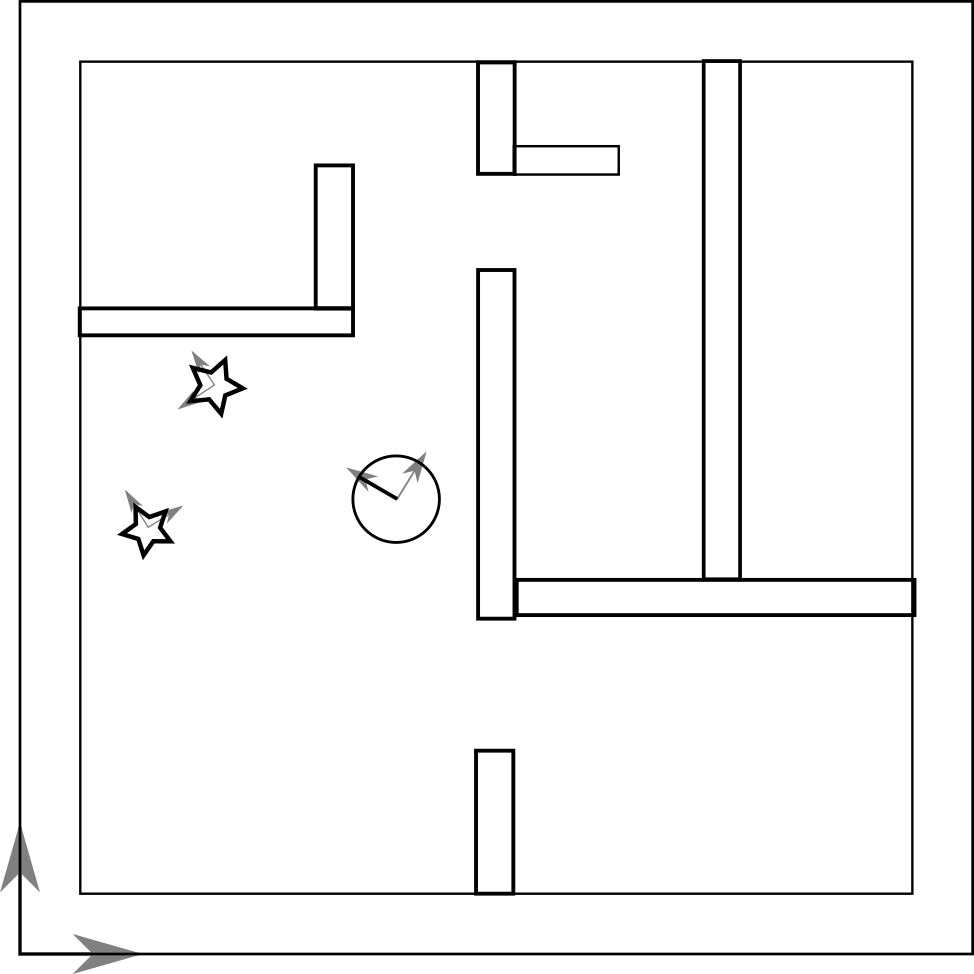
\includegraphics[width=8cm]{room}}	
\caption{部屋の中のロボット}
\label{fig:room}
\end{figure}

\begin{figure}[h] 
\centering{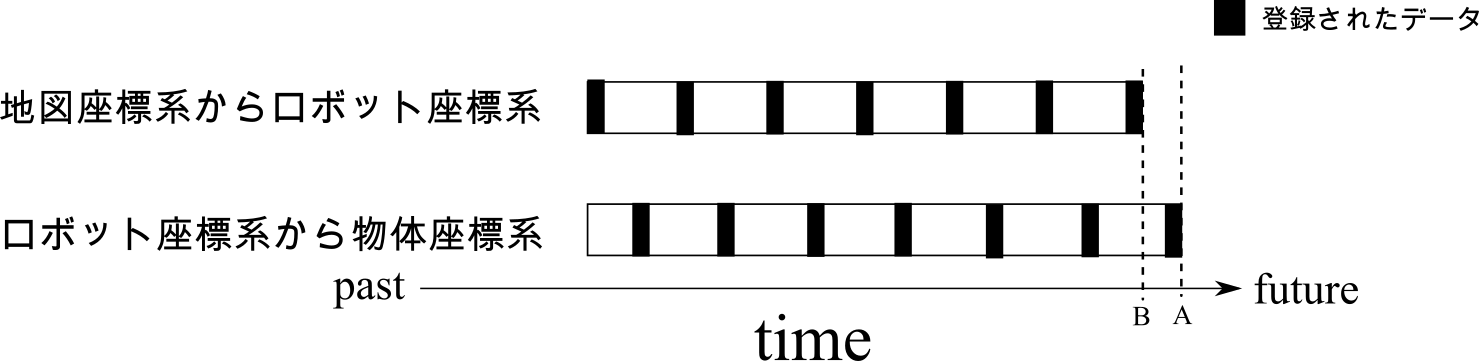
\includegraphics[width=10cm]{sensor-sync}}	
\caption{位置関係の登録のタイムライン}
\label{fig:sensor-sync}
\end{figure}


ここで地図中での物体の位置を把握するために、地図座標系から物体座標系への位置関係を取得する方法について考える。地図座標系から物体座標系への位置関係は地図座標系からロボット座標系への変換とロボット座標系から物体座標系への変換を掛け合わせれば計算ができるが、図\ref{fig:sensor-sync}のように各変換データは異なるタイミングで来るため、最新の変換データを取得するプログラムは複雑なものとなる。Aの時刻で地図座標系から物体座標系への変換データを計算しようとするとロボット座標系から物体座標系への最新の変換データを取得できるが、地図座標系からロボット座標系への変換データはまだ取得できない。このため、最新の変換データ$\theta$を取得する、もしくは過去のデータを元にデータの補外をすると必要がある。Bの時刻で地図座標系から物体座標系への変換データを計算しようとすると地図座標系からロボット座標系への最新の変換データを取得できるが、ロボット座標系から物体座標系への変換データはその時間には提供されていない。このため、$\alpha$と$\beta$のデータから線形補間を行う、もしくは最新の変換データ$\beta$を取得する必要がある。
また、地図座標系からロボット座標系への変換とロボット座標系から物体座標系への変換は別のプログラムで管理されており、座標系同士の変換に関する情報が分散している。

このように、ROSの開発初期には複数の座標変換の管理が開発者共通の悩みの種であると認識されていた。このタスクは複雑なために、開発者がデータに不適切な変換を適用した場合にバグが発生しやすい場所となっていた。また、この問題は異なる座標系同士の変換に関する情報が分散していることが多いことが課題となっていた。

そこで、TFライブラリは各座標系間の変換を有向森構造として一元管理し、効率的な座標系間の変換情報の登録、座標系間の変換の計算を可能にした。まず、図\ref{fig:room}を表す木構造は図\ref{fig:room-tree}で表現できる。木構造のノードが各座標系を表し、木構造のエッジは子ノードから親ノードへの変換データが存在することを表す。
% camera1, camera2の説明はいるだろうか?

\begin{figure}[h] 
\centering
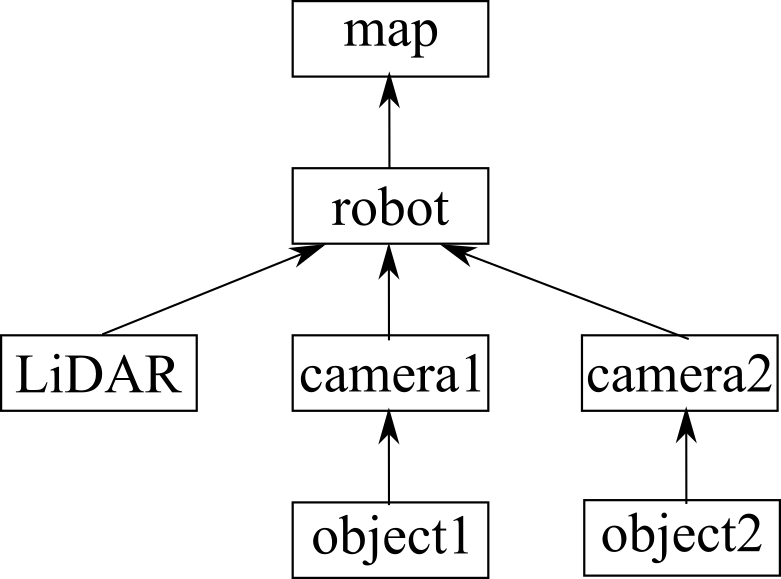
\includegraphics[width=10cm]{tree}	
\caption{図\ref{fig:room}に対応する木構造}
\label{fig:room-tree}
\end{figure}

各ノードはTFではフレームと呼ばれ、ノード中の文字列は各座標系に対応するフレーム名が書かれている。図\ref{fig:room-tree}では地図座標系のフレーム名はmap、ロボット座標系のフレーム名はrobot、物体1の座標系のフレーム名はobject1となる。木構造は子ノードから親ノードへポインタが貼られ、子ノードから親ノードを辿ることができる。このため、mapからobject1への座標変換を計算するにはobject1からmapへの座標変換の計算し、その逆数を取る必要がある。

子ノードから親ノードへの位置関係は子ノードが保持する。

先程説明したように、各フレーム間の座標変換情報はそれぞれ異なるタイミングで登録される。これに対処するため、TFでは各フレーム間の座標変換情報を過去一定期間保存する。図\ref{fig:room-tree}において各フレーム間の座標変換情報が登録されたタイミングを表すのが図\ref{fig:room-timeline}である。横軸は時間軸を表し、左側が過去、右側が最新の時刻を表す。黒色のセルはデータがその時刻にデータが登録されたことを表す。時刻Aではrobotからmapへの座標変換の情報が得られるが、object1からmapへの座標変換の情報は時刻Aには存在しない。そこで、TFでは前後のデータから線形補間を行うことにより該当する時刻の座標変換データを計算する。つまり、TFは該当する時刻の座標変換データが保存されている、もしくは前後の値を元に線形補間ができる場合にはその時刻の座標変換データを提供できる、とみなす。灰色の領域は線形補間により座標変換データが提供可能な時間領域を表す。

\begin{figure}[h] 
\centering
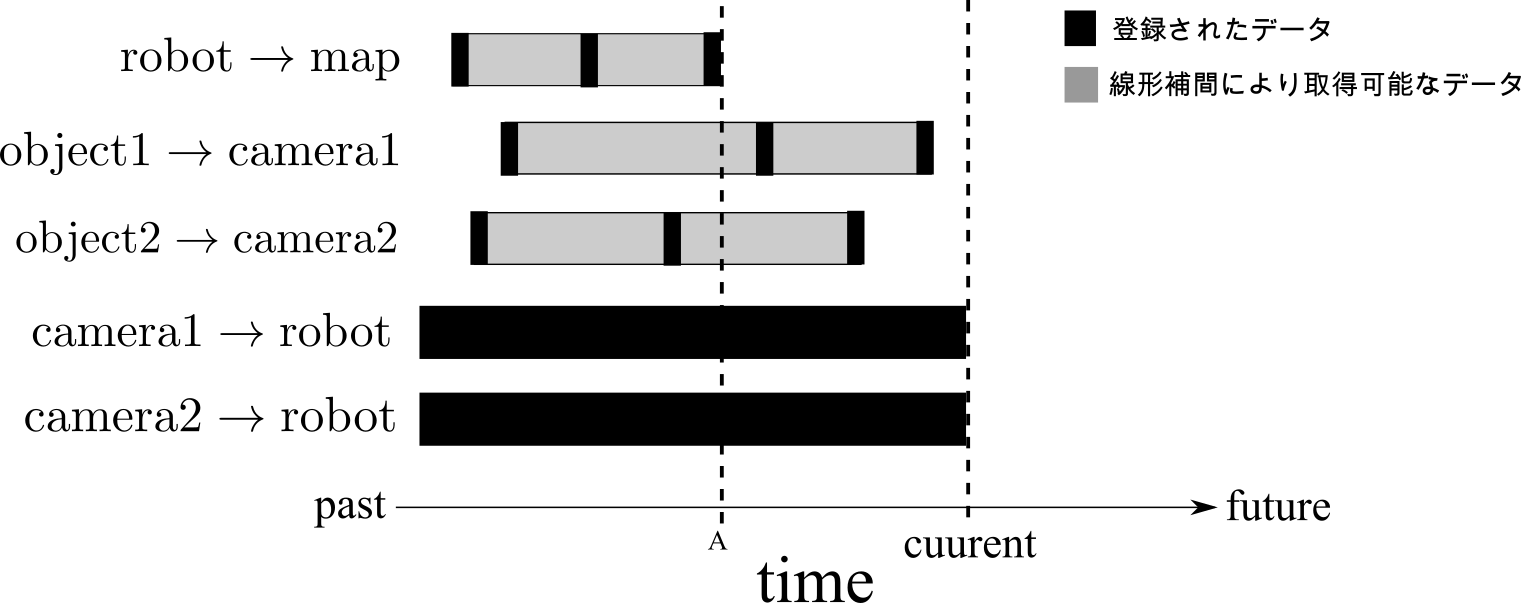
\includegraphics[width=10cm]{room-timeline}	
\caption{図\ref{fig:room-tree}における位置関係登録のタイムライン}
\label{fig:room-timeline}
\end{figure}

図\ref{fig:room-tree}における位置関係登録のタイムラインが図\ref{fig:room-timeline}のようになっているとき、TFではobject1からmapへの最新の位置関係は次のように計算する。

まず、object1からmapへのパスを確認する。ここではobject1からmapへのパスは$object1 \rightarrow camera1$, $camera1 \rightarrow robot$, $robot \rightarrow map$であることがわかる。

次に、どのパスにおいてもなるべく最新の座標変換を提供できる時刻を確認する。図\ref{fig:room-timeline}を確認すると、$object1 \rightarrow camera1$, $camera1 \rightarrow robot$, $robot \rightarrow map$において最新の座標変換情報が登録された時刻が最も古いのは$robot \rightarrow map$である。このため、時刻Aがここでは要件を満たす。

最後に、時刻Aでの各パスのデータを取得し、それらを掛け合わせる。$robot \rightarrow map$については登録されたデータを使い、$object1 \rightarrow camera1$, $camera1 \rightarrow robot$については線形補間によってデータを取得する。

\section{研究課題}
前述したようにTFはロボットシステム内部の座標系間の位置関係を一元管理する機構を提供する。しかしながら、これには以下のような問題点が挙げられる。

\subsection*{問題1:ジャイアント・ロック}
TFの森構造には複数のスレッドがアクセスするため並行性制御が必要となるが、既存のTFでは一つのスレッドが森構造にアクセスしている際は他のスレッドは森構造にアクセスできないアルゴリズムとなっている。これは、マルチコアが常識となっている現代では大きな問題となる。

\subsection*{問題2:データの鮮度}

上記の説明のように、TFのフレーム間の座標変換計算インターフェースは最新のデータを使わない可能性がある。同時刻のデータを元に座標変換を行うためデータの同期性はあるが、最新の座標変換データを使わないためデータの鮮度は失われる。現在、TFライブラリには最新の座標変換データをもとにフレーム間の座標変換計算をするインターフェイスは無い。

\section{研究方針}
前述した問題1については、データベースの並行性制御技術における細粒度ロッキング法を適用して解決する。細粒度ロッキング法は、並行性制御においてロックするデータの単位をなるべく小さくし、並行性を向上させる手法である。

問題2については、データベースのトランザクション技術における2PLを適用し、複数の座標変換の最新のデータをatomicに取得するインターフェース、及び複数の座標変換の最新のデータをatomicに更新するインターフェースを提供する。2PLとは、複数のデータに対するロック・アンロックのタイミングを二つのフェーズに分けることにより並行性を向上させつつデータ操作の一貫性を確保する手法である。

\section{貢献}

本研究ではデータベースのトランザクション技術における再粒度ロッキング法、及び並行性制アルゴリズムの一種である2PLを応用することにより、問題1および問題2を解決した。

\section{構成}
本論文の構成は次の通りである。第二章では関連研究について述べる。第三章では既存のTFの森構造とその問題点について述べる。第四章では提案手法である森構造への再粒度ロックの導入とデータ一貫性のためのインターフェイスの提供について述べる。第五章では提案手法の評価結果を述べる。第六章では本研究の結論を述べる。第七章では今後の課題について述べる。

\chapter{関連研究}
データベース分野におけるロボットの研究の例としてGAIA platform\cite{gaia}が挙げられる。


TFのようにデータを時系列的に管理するものとしてSSMが挙げられる。
% 移動ロボット用センサ情報処理ミドルウェアの開発 か?


データベースの技術をロボットに適用するという内容ではGAIA\cite{gaia}が挙げられる。
ロボットというより自律システム

C++に宣言的にデータ変更時のルールを記述できる。これによって簡単にイベントベース
trigger付きのUDFみたいな?

これはRDBベースでreactiveな挙動を提供する。


プロダクトレベルのものを目指すROS2\cite{ros2}やAutoware\cite{autoware}でも、livelinessなどの指標
DDS
が導入されたが、データベースの並行性制御の導入はない。



本研究のようなアプローチは存在しない。


2PL以外の並行性制御アルゴリズムとしてはSilo\cite{silo}が挙げられる。

% ここは後で書こうっと


\chapter{既存のTFの森構造とその問題点}
%TF森の実態はtf2パッケージ中にあるBufferCoreクラス\cite{buffer-core} である。
\section{構造}
TFライブラリでは図\ref{fig:multitree} のように各座標系間の位置関係を森構造で管理し、複数の木の登録が登録できる。ノードが各座標系を表し、エッジは子ノードから親ノードへの座標変換データが存在し、また子ノードから親ノードへポインタが貼られていることを表す。このため子ノードから親ノードへ辿ることはできるが、親ノードから子ノードを辿ることはできない。各ノードはフレームと呼ばれ、ノード内の文字列は各座標系に対応するフレーム名が書かれている。

各フレーム間の座標変換情報は過去10秒間保存される。このため、各フレーム間の座標変換情報が登録された時刻を図\ref{fig:general-timeline}のようなタイムラインで表現できる。黒のセルは登録されたデータを表し、灰色のセルは線形補間により座標変換データが取得可能な時刻を表す。横軸が時間軸を表し、左側が過去、右側が最新の時刻を表す。

\begin{figure}[h] 
\centering
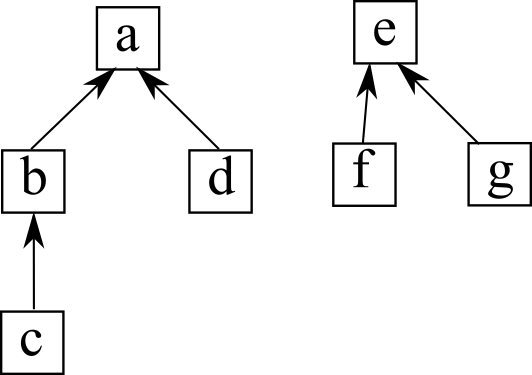
\includegraphics[width=7cm]{multitree.png}	
\caption{複数の木構造}
\label{fig:multitree}
\end{figure}

\begin{figure}[h] 
\centering
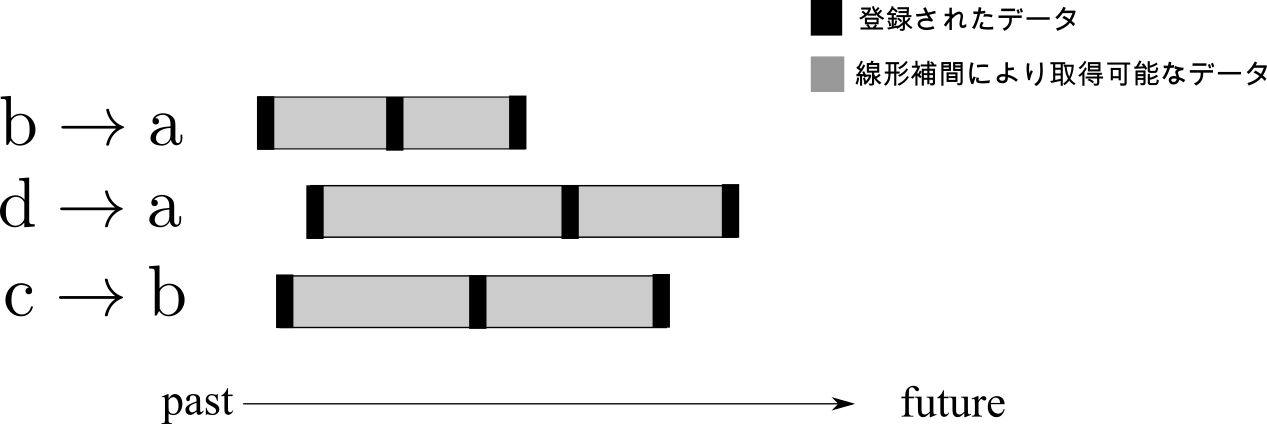
\includegraphics[width=10cm]{general-timeline.png}
\caption{タイムライン}
\label{fig:general-timeline}
\end{figure}


\section{lookupTransform}
二つのフレーム間の座標変換情報を取得するにはlookupTransformメソッドを使う。

登録されたフレームが図\ref{fig:multitree}、登録された座標変換情報のタイムラインが図\ref{fig:general-timeline}の状況において、lookupTransformメソッドを用いてフレームcからフレームdへの座標変換を計算するアルゴリズムを説明する。

\begin{enumerate}
	\item フレームcから木構造のルートノードへのパスを取得する。ここではルートノードはaとなり、フレームcからフレームaへのパスはc$\rightarrow$bとb$\rightarrow$aとなる。
	\item フレームdから木構造のルートノードへのパスを取得する。同じようにルートノードはaとなり、フレームdからフレームaへのパスはd$\rightarrow$aとなる。
	\item 得られた三つのどのパスにおいてもなるべく最新の座標変換を提供できる時刻を確認する。ここでは時刻Aが要件を満たす。
	\item 時刻Aにおける各パスの座標変換データを計算する。b$\rightarrow$aについては登録されたデータを利用でき、c$\rightarrow$bとd$\rightarrow$aについては線形補間されたデータを利用できる。
	\item フレームcからフレームaへの座標変換と、フレームaからdへの座標変換を掛け合わせる。フレームcからフレームaへの座標変換はc$\rightarrow$bとb$\rightarrow$aの座標変換をかけ合わせれば得られ、フレームaからdへの座標変換はd$\rightarrow$aの逆変換から得られる。
\end{enumerate}
% ショートカットについては説明不要?
% 途中で親が変わるケースはinsert/deleteが発生する場合に説明しよう
また、lookupTransformメソッドは指定した時刻のデータを取得することもできる。時刻Bにおけるフレームcからフレームdへの座標変換は次のアルゴリズムで得られる。

\begin{enumerate}
	\item フレームcから木構造のルートノードへの時刻Bにおける座標変換を取得する。フレームcから木構造のルートノードへのパスはc$\rightarrow$b、b$\rightarrow$aとなり、それぞれの座標変換は線形補間によって得られる。
	\item フレームdから木構造のルートノードへの時刻Bにおける座標変換を取得する。フレームdから木構造のルートノードへのパスはd$\rightarrow$aとなり、座標変換は線形補間によって得られる。
	\item フレームcからフレームaへの座標変換と、フレームaからdへの座標変換を掛け合わせる。フレームaからdへの座標変換はd$\rightarrow$aの逆変換から得られる。
\end{enumerate}

\section{setTransform}
二つのフレーム間の座標変換情報を更新するにはsetTransformメソッドを使う。図\ref{fig:multitree}におけるフレームcからフレームbのように直接の親子関係になっているフレーム間の座標変換情報を更新でき、フレームcからフレームaのように直接の親子関係になっていないフレーム間の座標変換情報は更新できない。フレームcからフレームaへの座標変換を更新するにはフレームcからフレームbへの座標変換、及びフレームbからフレームaへの座標変換を更新すればよい。

このメソッドを呼び出すことにより新しい座標変換情報がタイムラインに追加される。

% 図3.1においてc->aと貼り直すとbのdeleteが発生するが、ここではread/writeのみ扱うのでここでは記述しない。

\section{問題点}
\subsection*{問題1: ジャイアント・ロック}
TFライブラリの森構造で主に使われるインターフェイスは主にlookupTransformとsetTransformである。これらは複数のスレッドからアクセスされるので、並行性制御を行う必要があるが、TFライブラリではmutexを用いて森構造全体を保護している。このため、一つのスレッドが森構造にアクセスしている際は他のスレッドは森構造へのアクセスを待たされてしまう。これは、マルチコアが常識となっている現代では大きな問題となる。

\subsection*{問題2: データの鮮度}
森構造が図\ref{fig:multitree}、タイムラインが図\ref{fig:general-timeline}の状況において、lookupTransformを用いてフレームcからフレームdへの最新の座標変換を計算する時には時刻Aの時点での各フレーム間の座標変換データを用いる。この時、b$\rightarrow$aにおいては最新のデータを用いるが、c$\rightarrow$bにおいては最新のデータと一つ前のデータから線形補間されるデータを用いている。d$\rightarrow$aにおいては最新のデータ$\theta$ではなく一つ前のデータ$\alpha$とそのもう一つ前のデータ$\beta$から線形補間されるデータを用いている。このように、lookupTransformは二つのフレーム間の座標変換の計算において、フレーム間のパスの全てにおいて座標変換データを提供できる時刻についての座標変換を計算するという仕様のため、b$\rightarrow$aのように座標変換情報の登録が遅れるとそれに足を引っ張られてしまい、最新の座標変換データが使われなくなるという問題がある。時刻の同期をとっているためデータの同期性はあるが、最新のデータが使われなくなる可能性があり、データの鮮度は失われる。現在、TFライブラリには最新の座標変換データをもとにフレーム間の座標変換計算をするインターフェイスは無い。

\chapter{提案手法}
本研究では、データベースの並行性制御技術における細粒度ロッキング法及びトランザクション技術における2PLを適用し、これらの問題を解決する。

前述した問題1については、データベースの並行性制御技術における細粒度ロッキング法を適用して解決する。

図\ref{fig:giant-lock}の森構造においてスレッド1がlookupTransformを用いてフレームcからフレームaへの座標変換の計算、スレッド2がsetTransformを用いてフレームdからフレームaへの座標変換を更新する場合について考える。ここで、スレッド1はフレームcとフレームbのデータの読み込み、スレッド2はフレームdのデータの書き込みを行うため、スレッド$i$のデータ$x$に対する読み込み操作を$r_i(x)$、スレッド$i$のデータ$x$に対する書き込み操作を$w_i(x)$と表記すると、スレッド1の操作は$r_1(c)r_1(b)$、スレッド2の操作は$w_2(d)$と表記できる。


\begin{figure}[h] 
\centering
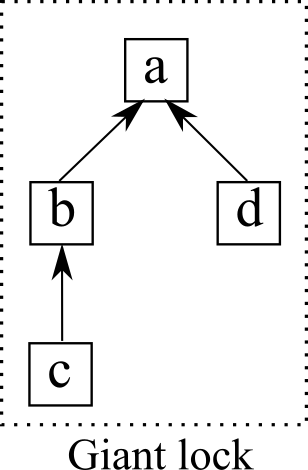
\includegraphics[width=4cm]{gaint-lock}	
\caption{Giant lock}
\label{fig:giant-lock}
\end{figure}


TFライブラリでは森構造へのアクセスをする際、森構造全体をジャイアント・ロックする。これにより、図\ref{fig:giant-lock}の点線枠部分が保護される。図\ref{fig:g-lock-time}はスレッド1の処理中にスレッド2の処理が開始した時のスケジューリングを図示している。セルが実行中の処理を表し、セルの端のGlockとGunlockは森構造へのジャイアントロック、アンロックを表す。スレッド2の処理が開始した時、スレッド1が森構造をジャイアントロックしているため、スレッド2はスレッド1の処理が完了し森構造のロックが外されるまで待機する必要がある。スレッド1がアクセスするデータとスレッド2がアクセスするデータは異なるため、より細かくロックする範囲を指定できる方法があればスレッド2がスレッド1の処理の完了を待つ必要がなくなる。


\begin{figure}[h] 
\centering
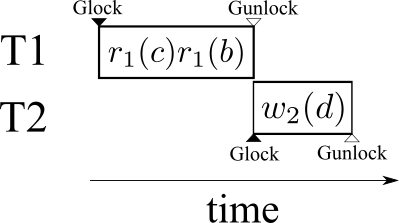
\includegraphics[width=7cm]{g-lock-time.png}	
\caption{ジャイアントロックにおけるスケジューリング}
\label{fig:g-lock-time}
\end{figure}

そこで、本研究ではデータベースの並行性制御技術における細粒度ロッキング法を適用する。
細粒度ロッキング法ではアクセスするデータにのみロックをかけ、さらにロックの種類を読み込みロックと書き込みロックに分ける。
複数のスレッドが同じデータにアクセスする際に発生するデータ競合を避けるために、排他制御では一つのスレッドからのみデータにアクセスできるようにするため、ロックをかける。しかしながら、複数のスレッドが同じデータにアクセスする際、データの読み込みのみ行うのであればデータ競合は発生しない。そこで、データの読み込みのみを行う時には読み込みロック、データの書き込みを行う時には書き込みロックを使い、次のようなルールを設ける。

\begin{itemize}
 \item 読み込みを行う前に読み込みロック、書き込みを行う前に書き込みロックを行う必要がある
 \item ロックされていないデータには読み込みロック、及び書き込みロックをかけられる
 \item すでに読み込みロックされたデータにも他のスレッドが読み込みロックをかけることができる
 \item すでに読み込みロックされたデータには他のスレッドが書き込みロックをかけることはできない
 \item すでに書き込みロックされたデータには他のスレッドが読み込みロックも書き込みロックもかけることはできない
\end{itemize}


\begin{table}[h!]
\centering
\begin{tabular}{ | m{1cm} | m{1cm} | m{1cm} | } 
  \hline
  & $rl_i(x)$ & $wl_i(x)$ \\ 
  \hline
  $rl_j(x)$ & $\circ$ & $\times$ \\ 
  \hline
  $wl_j(x)$ &  $\times$ & $\times$ \\ 
  \hline
\end{tabular}	
\caption{lock table}
\label{table:lock-table}
\end{table}


このルールは、表\ref{table:lock-table}のような表形式で説明することもできる。表中ではスレッド$i$のデータ$x$に対する読み込みロック操作を$rl_i(x)$、スレッド$i$のデータ$x$に対する書き込みロック操作を$wl_i(x)$と表記する。表は一行目がスレッド$i$によってロックがかけられている状態を表し、その状態に読み込みロック、または書き込みロックをスレッド$j$がかけられるかどうかを2、3行目で表している。$\circ$はすでにロックがかかっていても別のスレッドがロックをかけられることを表し、$\times$はそうでないことを表す。例えば、2行2列目はすでに$rl_i(x)$がかかっていても$rl_j(x)$がかけられることを表し、2行3列目はすでに$wl_i(x)$がかかっていると$rl_j(x)$はかけられないことを表す。

\begin{figure}[h] 
\centering
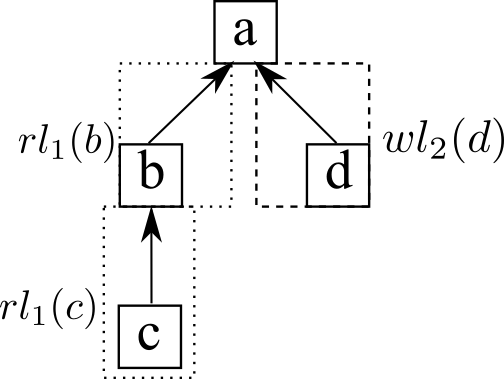
\includegraphics[width=7cm]{high-gran-lock}
\caption{細粒度ロッキング}
\label{fig:high-gran-lock}
\end{figure}


\begin{figure}[h] 
\centering
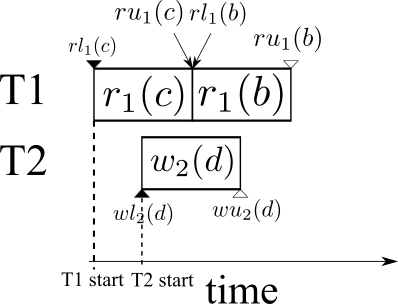
\includegraphics[width=7cm]{high-gran-time}
\caption{細粒度ロックにおけるスケジューリング}
\label{fig:high-gran-time}
\end{figure}



細粒度ロッキングを用いた場合のスレッド1、スレッド2の保護範囲は図\ref{fig:high-gran-lock}、スケジューリングは図\ref{fig:high-gran-time}で表せる。図\ref{fig:high-gran-time}ではスレッド$i$がデータ$x$を読み込みアンロック、書き込みアンロックする時にはそれぞれ$ru_i(x), wu_i(x)$と表記される。

スレッド1の実行中にスレッド2の処理が開始しても、図\ref{fig:high-gran-lock}で表されるようにスレッド1とスレッド2でアクセスするデータは異なるため、スレッド2はスレッド1の処理完了を待機する必要がなくなる。


\begin{figure}[h] 
\centering
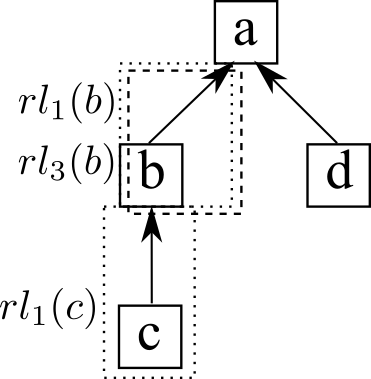
\includegraphics[width=5cm]{two-read-lock}
\caption{二つの読み込みロック}
\label{fig:two-read-lock}
\end{figure}


\begin{figure}[h] 
\centering
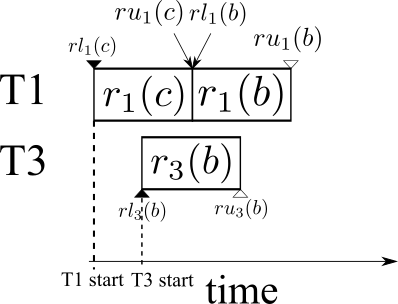
\includegraphics[width=7cm]{two-read-lock-time}
\caption{二つの読み込みロックにおけるスケジューリング}
\label{fig:two-read-lock-time}
\end{figure}

スレッド1の処理の途中に、lookupTransformを用いてフレームdのデータを読み込むスレッド3が開始するケースについて考える。細粒度ロッキングを用いた場合のスレッド1とスレッド3の保護範囲は図\ref{fig:two-read-lock}で、スケジューリングは図\ref{fig:two-read-lock-time}で表記される。スレッド1にてデータbに対して読み込みロックを取るときすでにスレッド3がbを読み込みロックしているが、表\ref{table:lock-table}が表すようにすでに読み込みロックがかけられていても他のスレッドが読み込みロックをかけることができる。


このように、細粒度ロッキング法ではデータごとにロックをし、さらに読み込みロック・書き込みロックと区別をつけることにより並行性を上げることができる。


前述した問題2については、複数の座標変換のデータをatomicに取得するインターフェース(lookupLatestTransform)、及び複数の座標変換の最新のデータをatomicに更新するインターフェース(setTransforms)を提供して解決する。setTransformsインターフェイスの必要性について説明する。

まず、二つのフレーム間の座標変換を計算する際に線形補間を行わずにフレーム間のパスの最新の座標変換データを使うインターフェイスとしてlookupLatestTransformを導入する。これは森構造が図\ref{fig:multitree}、タイムラインが図\ref{fig:general-timeline}における状況でフレームcからフレームdへの座標変換は次のように計算される。

\begin{enumerate}
	\item フレームcから木構造のルートノードへパスをたどりながら、各フレーム間の最新の座標変換を掛け合わせてフレームから木構造のルートノードへの座標変換を計算する。ここでは、フレームcから木構造のルートノードへのパスはc$\rightarrow$b、b$\rightarrow$aとなり、それぞれの座標変換は最新のものを使う。
	\item 同じように、フレームdから木構造のルートノードへパスをたどりながら、各フレーム間の最新の座標変換を掛け合わせてフレームから木構造のルートノードへの座標変換を計算する。
	\item フレームcから木構造のルートノードへの座標変換と、木構造のルートノードからフレームdへの座標変換を掛け合わせる。木構造のルートノードからフレームdへの座標変換はフレームdから木構造のルートノードへの座標変換の逆変換から得られる。
\end{enumerate}

\begin{figure}[h] 
\centering
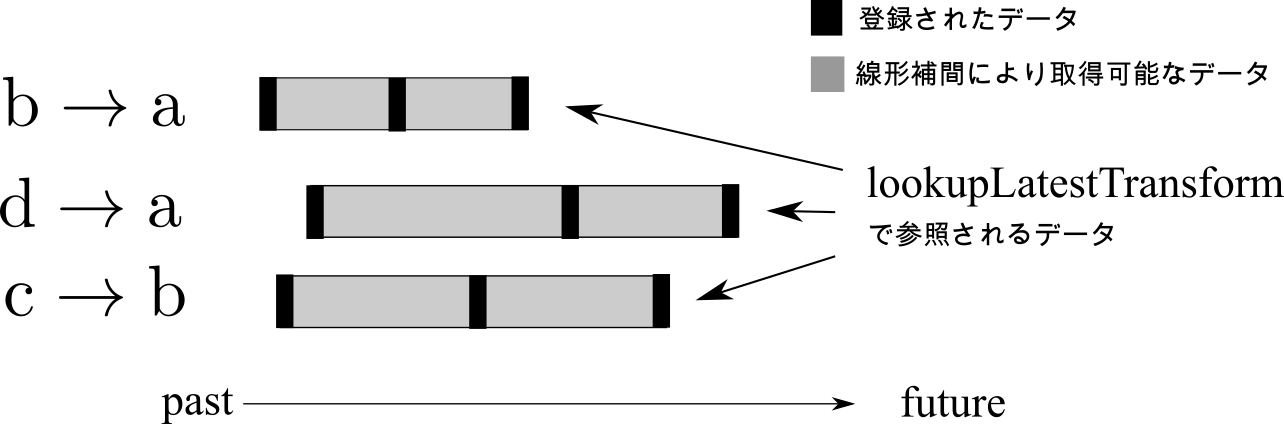
\includegraphics[width=12cm]{lookupLatestTransform}
\caption{lookupLatestTransformで取得するデータ}
\label{fig:lookupLatestTransform}
\end{figure}

lookupLatestTransformにて取得する座標変換データは、図\ref{fig:lookupLatestTransform}のように図示できる。


しかしながら次の問題が生じる

ここで
つまり両方が2PLじゃないと



続いて、最新のデータを取らない問題と線形補間によりデータの一貫性がなくなる問題について

既存のlookupTransformでは、最新のデータを取得しようとしても過去のデータを参照してしまう、また線形補間されてしまう

最新のデータをそれぞれ取ってくるという方法もサポートする。(しかしこれだけでは十分ではない。 <- この導入はいまいち。)冒頭で説明したように、ROSは分散アーキテクチャを採用する。TFMessageには各フレーム間の座標変換情報を複数登録できるが、TFは複数の座標変換をsetTransformを複数回呼び出すことにより実現している。これにより、中間の状態を見てしまう。これは図のように説明できる。
この図のように、giant lockを毎回のsetTransformで取ってはいるが、その操作が終わり次のsetTransformsを呼ぶまでの間はlockが外される。これにより、一貫性のない状態を見てしまう恐れがある。


そこで、我々は最新のデータをatomicに取得するlookupLatestTransform、及び複数の座標変換を一度にatomicに登録できるseTransformsを追加した。複数のデータに対する読み込み、書き込みをatomicに行うために、我々は2PL[?]を実装した。

しかしながら2PLにはdead lockの問題がある。
例えば次の例、これは木を登る方向と下る方向の両方があるからこうなる。

データをreorderできれば2PLではdeadlockは発生しない(DAGが構築できる)、がTF木ではできそうにない。

そこで我々はdeadlock preventの方法としてNo-wait[Bern 1981]を採用した。これはwrite lockをかけようとして失敗したら最初からやり直す。

Wound wait, nonpreemptive (Concurrency Control in Distributed Database Systems PHLIP.A BERNSTEIN AND NATHAN GOODMAN P196)

transactionにpriorityを足すとかは?



\chapter{評価}
実験を行う

スレッド数を上げるとスループット伸びる
jointを増やすと緩やかにスループットが落ちる
iterを増やすと1000以降で急激にスループットが下がる。no waitによる弊害か?lockの確保に失敗しているのかも
read ratioは高くなるほどブロックされる可能性が減る
read lenは安定しているように見える。なぜtrnでread lenが小さいとこうなるのか。。。2PLでロックする箇所が変わるから?

write lenを上げるとやはりブロックされる部分が増える



56以上で下がる理由としてはROS timeとか
ここはインターフェイスでは…的な話


\chapter{結論}
再粒度ロックの導入により、パフォーマンスを上げることができた
特に、スレッド数の増加とともにスループットが下がる問題を解決できた

データの一貫性は必須、というデータも示したい。

\chapter{今後の課題}
ここでは取り上げなかったTF木の問題点として、部分的に座標情報の登録に失敗するケース。rollbackなどもいれtransactionalに行う必要

また、insert/deleteが大量に発生するケースも考える。


\chapter*{謝辞}
\addcontentsline{toc}{chapter}{\numberline{}謝辞}

本研究を進めるにあたり、慶應義塾大学准教授川島英之先生とサイボウズラボ株式会社星野喬様に頂きました優れた御指導により、私の研究はとても有意義で満ち足りたものとなりました。また、慶應義塾大学川島研究会秘書藤川綾様には幾多の手続きを丁寧にサポートして頂き,円滑な出張や書類作成,研究環境整備を行うことができました。そして、CCBench開発者である株式会社ノーチラス・テクノロジーズ田辺敬之様。この研究に関わっていただいたすべての方に深く感謝を申し上げます。

% 参考文献(References)
\newpage
\addcontentsline{toc}{chapter}{\numberline{}参考文献}
\renewcommand{\bibname}{参考文献}



%% 参考文献に bibtex を使う場合
%\bibliographystyle{junsrt}
%\bibliography{ref}

%% 参考文献を直接ファイルに含めて書く場合
	
\begin{thebibliography}{99}


\bibitem{ros} M. Quigley, K. Conley, B. P. Gerkey, J. Faust, T. Foote, J. Leibs, R. Wheeler, and A. Y. Ng, “Ros: an open-source robot operating system,” in ICRA Workshop on Open Source Software, 2009.

\bibitem{tf} T. Foote, "tf: The transform library," 2013 IEEE Conference on Technologies for Practical Robot Applications (TePRA), 2013, pp. 1-6, doi: 10.1109/TePRA.2013.6556373.

\bibitem{2PL} Philip A. Bernstein and Nathan Goodman, "Concurrency Control in Distributed Database Systems" in ACM Computing Surveys, 1981, pp. 185-221

\bibitem{buffer-core} "BufferCore.h", \url{https://github.com/ros/geometry2/blob/noetic-devel/tf2/include/tf2/buffer_core.h}

\bibitem{gaia} "GAIA platform", \url{https://www.gaiaplatform.io}

\bibitem{ros2} "ROS2", \url{https://docs.ros.org/en/rolling/}

\bibitem{autoware} "Autoware", \url{https://tier4.jp/en/autoware/}

\bibitem{silo} Stephen Tu, Wenting Zheng, Eddie Kohler †, Barbara Liskov,
and Samuel Madden. Speedy transactions in multicore in-memory
databases. In SOSP, pages 18–32. ACM, 2013

\end{thebibliography}


\end{document}
